% Options for packages loaded elsewhere
\PassOptionsToPackage{unicode}{hyperref}
\PassOptionsToPackage{hyphens}{url}
%
\documentclass[
]{article}
\usepackage{amsmath,amssymb}
\usepackage{lmodern}
\usepackage{iftex}
\ifPDFTeX
  \usepackage[T1]{fontenc}
  \usepackage[utf8]{inputenc}
  \usepackage{textcomp} % provide euro and other symbols
\else % if luatex or xetex
  \usepackage{unicode-math}
  \defaultfontfeatures{Scale=MatchLowercase}
  \defaultfontfeatures[\rmfamily]{Ligatures=TeX,Scale=1}
\fi
% Use upquote if available, for straight quotes in verbatim environments
\IfFileExists{upquote.sty}{\usepackage{upquote}}{}
\IfFileExists{microtype.sty}{% use microtype if available
  \usepackage[]{microtype}
  \UseMicrotypeSet[protrusion]{basicmath} % disable protrusion for tt fonts
}{}
\makeatletter
\@ifundefined{KOMAClassName}{% if non-KOMA class
  \IfFileExists{parskip.sty}{%
    \usepackage{parskip}
  }{% else
    \setlength{\parindent}{0pt}
    \setlength{\parskip}{6pt plus 2pt minus 1pt}}
}{% if KOMA class
  \KOMAoptions{parskip=half}}
\makeatother
\usepackage{xcolor}
\usepackage[margin=1in]{geometry}
\usepackage{longtable,booktabs,array}
\usepackage{calc} % for calculating minipage widths
% Correct order of tables after \paragraph or \subparagraph
\usepackage{etoolbox}
\makeatletter
\patchcmd\longtable{\par}{\if@noskipsec\mbox{}\fi\par}{}{}
\makeatother
% Allow footnotes in longtable head/foot
\IfFileExists{footnotehyper.sty}{\usepackage{footnotehyper}}{\usepackage{footnote}}
\makesavenoteenv{longtable}
\usepackage{graphicx}
\makeatletter
\def\maxwidth{\ifdim\Gin@nat@width>\linewidth\linewidth\else\Gin@nat@width\fi}
\def\maxheight{\ifdim\Gin@nat@height>\textheight\textheight\else\Gin@nat@height\fi}
\makeatother
% Scale images if necessary, so that they will not overflow the page
% margins by default, and it is still possible to overwrite the defaults
% using explicit options in \includegraphics[width, height, ...]{}
\setkeys{Gin}{width=\maxwidth,height=\maxheight,keepaspectratio}
% Set default figure placement to htbp
\makeatletter
\def\fps@figure{htbp}
\makeatother
\setlength{\emergencystretch}{3em} % prevent overfull lines
\providecommand{\tightlist}{%
  \setlength{\itemsep}{0pt}\setlength{\parskip}{0pt}}
\setcounter{secnumdepth}{-\maxdimen} % remove section numbering
\usepackage{booktabs}
\usepackage{longtable}
\usepackage{array}
\usepackage{multirow}
\usepackage{wrapfig}
\usepackage{float}
\usepackage{colortbl}
\usepackage{pdflscape}
\usepackage{tabu}
\usepackage{threeparttable}
\usepackage{threeparttablex}
\usepackage[normalem]{ulem}
\usepackage{makecell}
\usepackage{xcolor}
\ifLuaTeX
  \usepackage{selnolig}  % disable illegal ligatures
\fi
\IfFileExists{bookmark.sty}{\usepackage{bookmark}}{\usepackage{hyperref}}
\IfFileExists{xurl.sty}{\usepackage{xurl}}{} % add URL line breaks if available
\urlstyle{same} % disable monospaced font for URLs
\hypersetup{
  pdftitle={Untitled},
  pdfauthor={Rimjhim Saxena},
  hidelinks,
  pdfcreator={LaTeX via pandoc}}

\title{Untitled}
\author{Rimjhim Saxena}
\date{2023-03-03}

\begin{document}
\maketitle

Loading data

Panel regression - by Job Sector

\tiny

\begin{longtable}[]{@{}
  >{\raggedright\arraybackslash}p{(\columnwidth - 10\tabcolsep) * \real{0.3511}}
  >{\centering\arraybackslash}p{(\columnwidth - 10\tabcolsep) * \real{0.1383}}
  >{\centering\arraybackslash}p{(\columnwidth - 10\tabcolsep) * \real{0.1489}}
  >{\centering\arraybackslash}p{(\columnwidth - 10\tabcolsep) * \real{0.1383}}
  >{\centering\arraybackslash}p{(\columnwidth - 10\tabcolsep) * \real{0.1064}}
  >{\centering\arraybackslash}p{(\columnwidth - 10\tabcolsep) * \real{0.1170}}@{}}
\caption{Sector Realloacation}\tabularnewline
\toprule()
\begin{minipage}[b]{\linewidth}\raggedright
\end{minipage} & \begin{minipage}[b]{\linewidth}\centering
Agriculture
\end{minipage} & \begin{minipage}[b]{\linewidth}\centering
Construction
\end{minipage} & \begin{minipage}[b]{\linewidth}\centering
Manufacture
\end{minipage} & \begin{minipage}[b]{\linewidth}\centering
Mining
\end{minipage} & \begin{minipage}[b]{\linewidth}\centering
Service
\end{minipage} \\
\midrule()
\endfirsthead
\toprule()
\begin{minipage}[b]{\linewidth}\raggedright
\end{minipage} & \begin{minipage}[b]{\linewidth}\centering
Agriculture
\end{minipage} & \begin{minipage}[b]{\linewidth}\centering
Construction
\end{minipage} & \begin{minipage}[b]{\linewidth}\centering
Manufacture
\end{minipage} & \begin{minipage}[b]{\linewidth}\centering
Mining
\end{minipage} & \begin{minipage}[b]{\linewidth}\centering
Service
\end{minipage} \\
\midrule()
\endhead
tmax & 4.1149** & -0.3492 & -1.1366+ & -0.2659 & -4.7253** \\
& (1.5427) & (0.2473) & (0.6029) & (0.6977) & (1.7705) \\
Num.Obs. & 2016 & 1803 & 1890 & 576 & 2018 \\
R2 & 0.450 & 0.387 & 0.601 & 0.711 & 0.369 \\
R2 Adj. & 0.309 & 0.208 & 0.493 & 0.475 & 0.209 \\
RMSE & 13.47 & 4.36 & 5.35 & 2.50 & 11.04 \\
FE: as.factor(State\_District\_72) & X & X & X & X & X \\
\bottomrule()
\end{longtable}

\textbf{Note:} \^{}\^{} + p \textless{} 0.1, * p \textless{} 0.05, ** p
\textless{} 0.01, *** p \textless{} 0.001

\begin{longtable}[]{@{}
  >{\raggedright\arraybackslash}p{(\columnwidth - 10\tabcolsep) * \real{0.3438}}
  >{\centering\arraybackslash}p{(\columnwidth - 10\tabcolsep) * \real{0.1354}}
  >{\centering\arraybackslash}p{(\columnwidth - 10\tabcolsep) * \real{0.1458}}
  >{\centering\arraybackslash}p{(\columnwidth - 10\tabcolsep) * \real{0.1354}}
  >{\centering\arraybackslash}p{(\columnwidth - 10\tabcolsep) * \real{0.1146}}
  >{\centering\arraybackslash}p{(\columnwidth - 10\tabcolsep) * \real{0.1250}}@{}}
\caption{Sector Realloacation}\tabularnewline
\toprule()
\begin{minipage}[b]{\linewidth}\raggedright
\end{minipage} & \begin{minipage}[b]{\linewidth}\centering
Agriculture
\end{minipage} & \begin{minipage}[b]{\linewidth}\centering
Construction
\end{minipage} & \begin{minipage}[b]{\linewidth}\centering
Manufacture
\end{minipage} & \begin{minipage}[b]{\linewidth}\centering
Mining
\end{minipage} & \begin{minipage}[b]{\linewidth}\centering
Service
\end{minipage} \\
\midrule()
\endfirsthead
\toprule()
\begin{minipage}[b]{\linewidth}\raggedright
\end{minipage} & \begin{minipage}[b]{\linewidth}\centering
Agriculture
\end{minipage} & \begin{minipage}[b]{\linewidth}\centering
Construction
\end{minipage} & \begin{minipage}[b]{\linewidth}\centering
Manufacture
\end{minipage} & \begin{minipage}[b]{\linewidth}\centering
Mining
\end{minipage} & \begin{minipage}[b]{\linewidth}\centering
Service
\end{minipage} \\
\midrule()
\endhead
temp\_effective & 5.5216*** & -0.0340*** & -0.1489*** & -0.0983** &
-0.3838*** \\
& (0.3654) & (0.0050) & (0.0308) & (0.0363) & (0.0524) \\
Num.Obs. & 2016 & 1803 & 1890 & 576 & 2018 \\
R2 & 0.598 & 0.402 & 0.607 & 0.715 & 0.394 \\
R2 Adj. & 0.496 & 0.228 & 0.500 & 0.482 & 0.240 \\
RMSE & 11.51 & 4.31 & 5.31 & 2.48 & 10.82 \\
FE: as.factor(State\_District\_72) & X & X & X & X & X \\
\bottomrule()
\end{longtable}

\textbf{Note:} \^{}\^{} + p \textless{} 0.1, * p \textless{} 0.05, ** p
\textless{} 0.01, *** p \textless{} 0.001

Panel regression - by Exposure

\begin{longtable}[]{@{}lcc@{}}
\caption{Sector Realloacation}\tabularnewline
\toprule()
& Exposed & Insular \\
\midrule()
\endfirsthead
\toprule()
& Exposed & Insular \\
\midrule()
\endhead
temp\_effective & -0.0008 & -0.0246 \\
& (0.0008) & (0.0685) \\
Num.Obs. & 6285 & 2018 \\
R2 & 0.750 & 0.746 \\
R2 Adj. & 0.702 & 0.489 \\
RMSE & 6.66 & 7.00 \\
FE: as.factor(State\_District\_72) & X & X \\
FE: as.factor(round) & X & X \\
FE: as.factor(State\_Region)\^{}as.factor(round) & X & X \\
\bottomrule()
\end{longtable}

\textbf{Note:} \^{}\^{} + p \textless{} 0.1, * p \textless{} 0.05, ** p
\textless{} 0.01, *** p \textless{} 0.001

\hypertarget{ag---nonag}{%
\section{Ag - NonAg}\label{ag---nonag}}

\tiny

\begin{longtable}[]{@{}lcc@{}}
\caption{Sector Realloacation - Ag/Non Ag}\tabularnewline
\toprule()
& 0 & 1 \\
\midrule()
\endfirsthead
\toprule()
& 0 & 1 \\
\midrule()
\endhead
temp\_effective & 0.0009 & -0.1525 \\
& (0.0012) & (1.4381) \\
Num.Obs. & 6277 & 2010 \\
R2 & 0.757 & 0.759 \\
R2 Adj. & 0.734 & 0.668 \\
RMSE & 8.60 & 8.88 \\
FE: State\_District\_72 & X & X \\
FE: as.factor(State)\^{}as.factor(round) & X & X \\
\bottomrule()
\end{longtable}

\textbf{Note:} \^{}\^{} + p \textless{} 0.1, * p \textless{} 0.05, ** p
\textless{} 0.01, *** p \textless{} 0.001

\begin{verbatim}
## `geom_smooth()` using formula = 'y ~ x'
\end{verbatim}

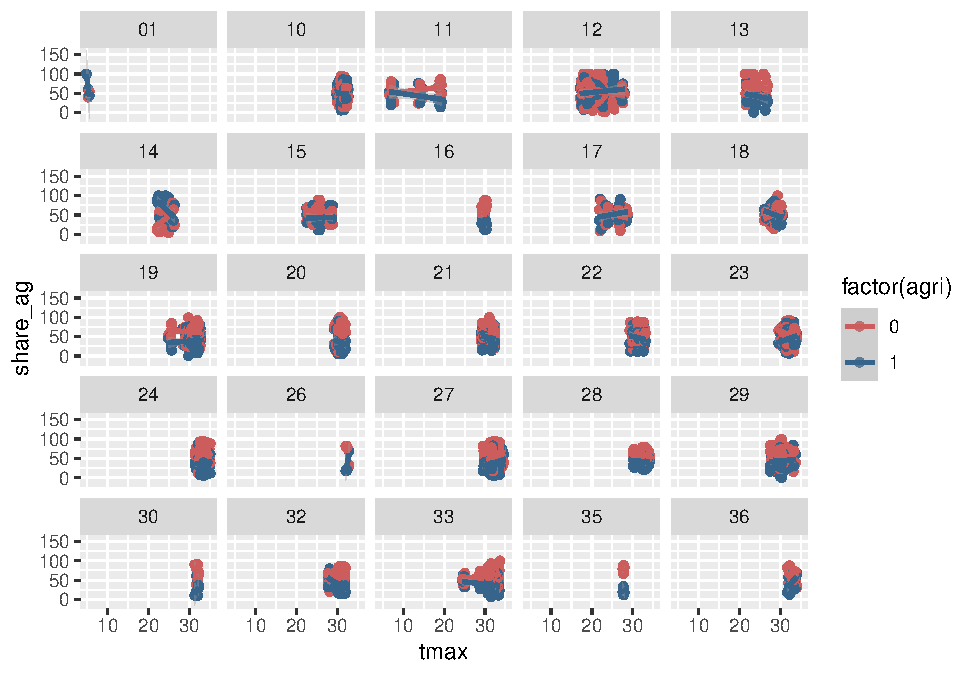
\includegraphics{09panel-regs_files/figure-latex/unnamed-chunk-9-1.pdf}

\begin{verbatim}
## `geom_smooth()` using formula = 'y ~ x'
\end{verbatim}

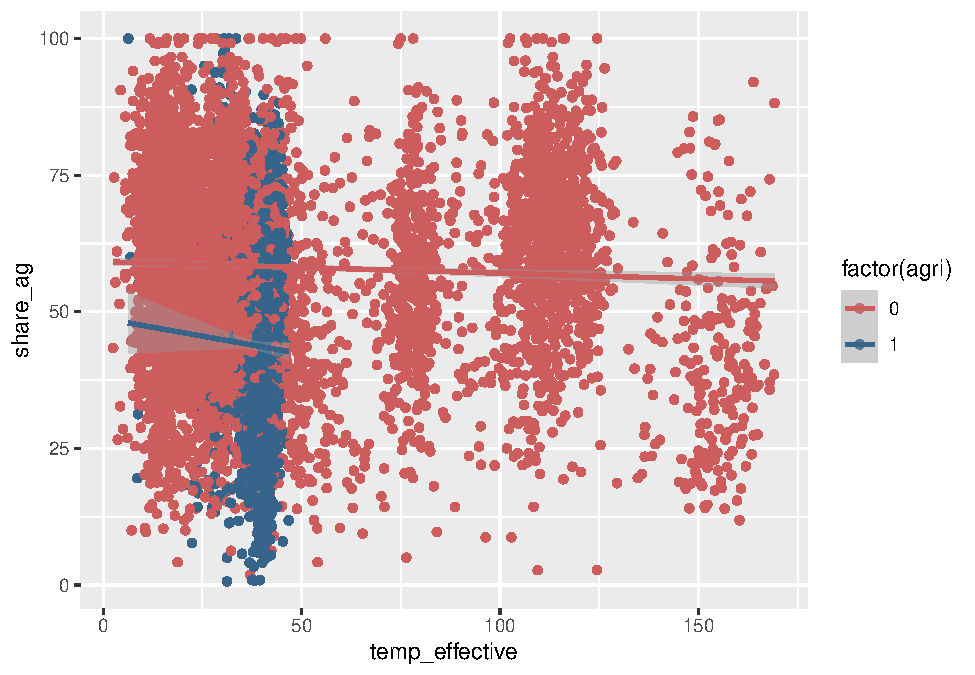
\includegraphics{09panel-regs_files/figure-latex/unnamed-chunk-9-2.pdf}

\end{document}
